\begin{figure}[htbp]
    \centering
    \begin{subfigure}[b]{0.49\textwidth}
        \centering
        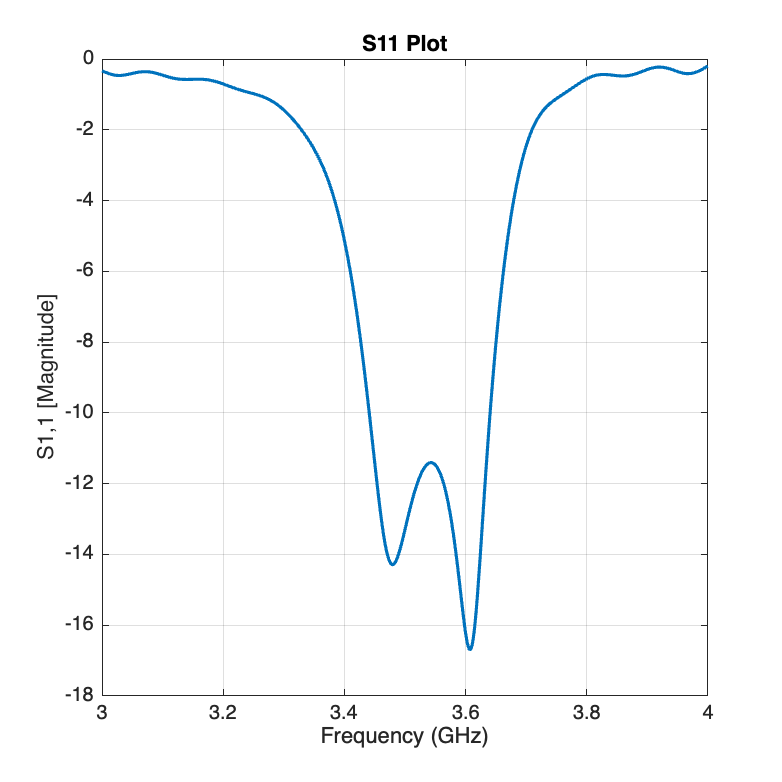
\includegraphics[width=\textwidth]{images/antenna/S11.png}
        \caption{S-parameters of Antenna}
        \label{fig:antenna_s}
    \end{subfigure}
    \hfill % horizontal space between subfigures
    \begin{subfigure}[b]{0.49\textwidth}
        \centering
        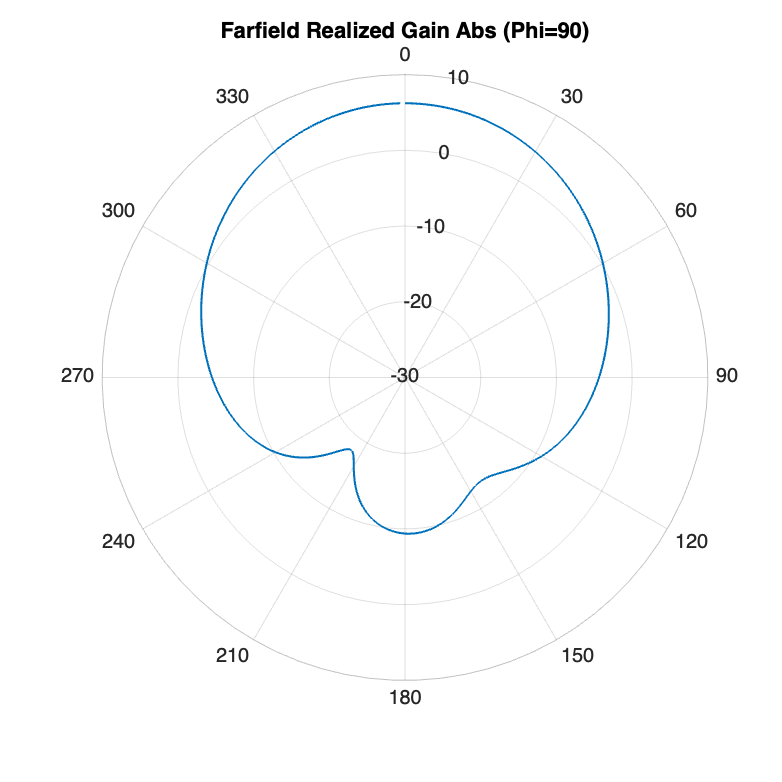
\includegraphics[width=\textwidth]{images/antenna/FF_p.png}
        \caption{Far Field Distribution}
        \label{fig:antenna_ff}
    \end{subfigure}
    \caption{Antenna Outputs}
    \label{fig:ant}
\end{figure}


\begin{comment}
\begin{figure}
    \centering
    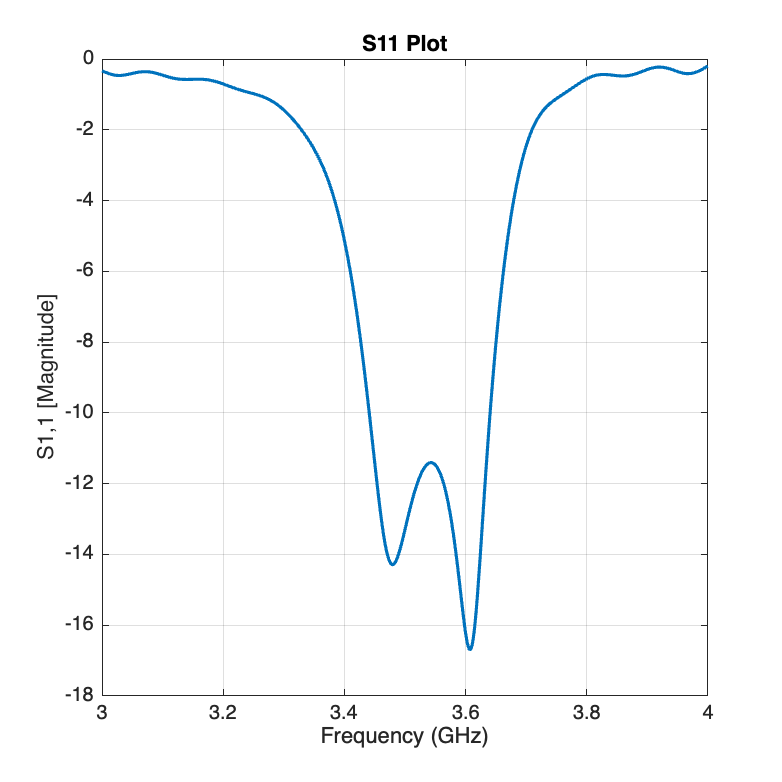
\includegraphics[width=0.8\textwidth]{images/antenna/S11.png}
    \caption{S-parameters of Antenna}
    \label{fig:antenna_s}
\end{figure}

\begin{figure}
    \centering
    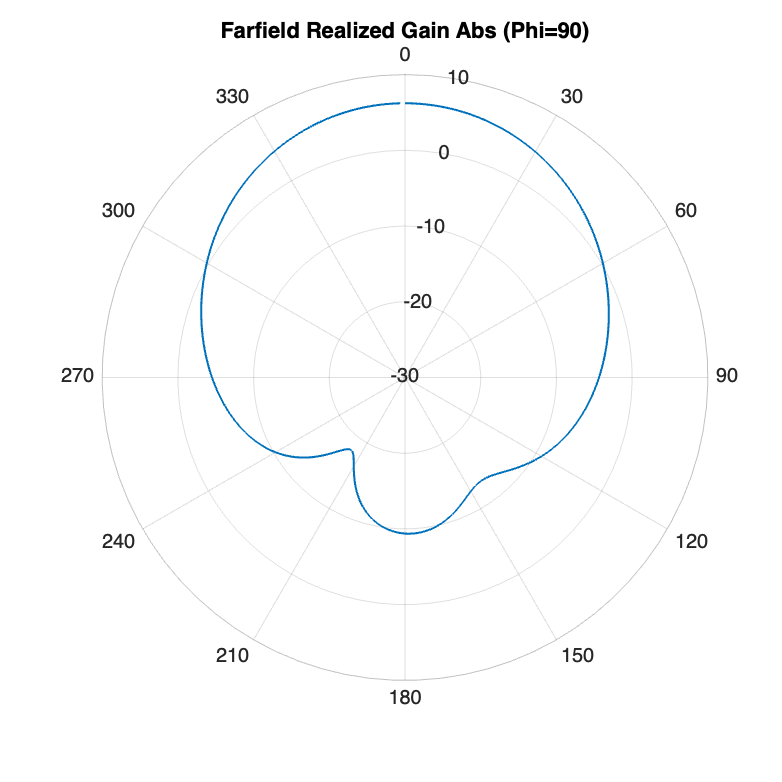
\includegraphics[width=0.8\textwidth]{images/antenna/FF_p.png}
    \caption{Far Field Distribution}
    \label{fig:antenna_ff}
\end{figure}
\end{comment}

The far-field characteristics of the microstrip patch antenna seen in Figure (\ref{fig:antenna_ff}) and Table (\ref{table:antenna_characteristics}), having a main lobe magnitude of \(6.22 [dBi]\), a side lobe level of \(-15.6 [dBi]\), and an angular width of \(79.9 \deg\) at \(3 [dB]\), demonstrate typical performance metrics for such antennas, indicating efficient radiation and low interference from side lobes.


\textbf{Fabrication:}
The circuit, matching network and antenna were layed out in Altium and sent for fabrication. CST-provided specs were used when deciding the board dimensions, so as to preclude fringing affects. The final layout of just the circuit section is seen in Figure (\(\ref{fig:board}\)).
\begin{figure}
    \centering
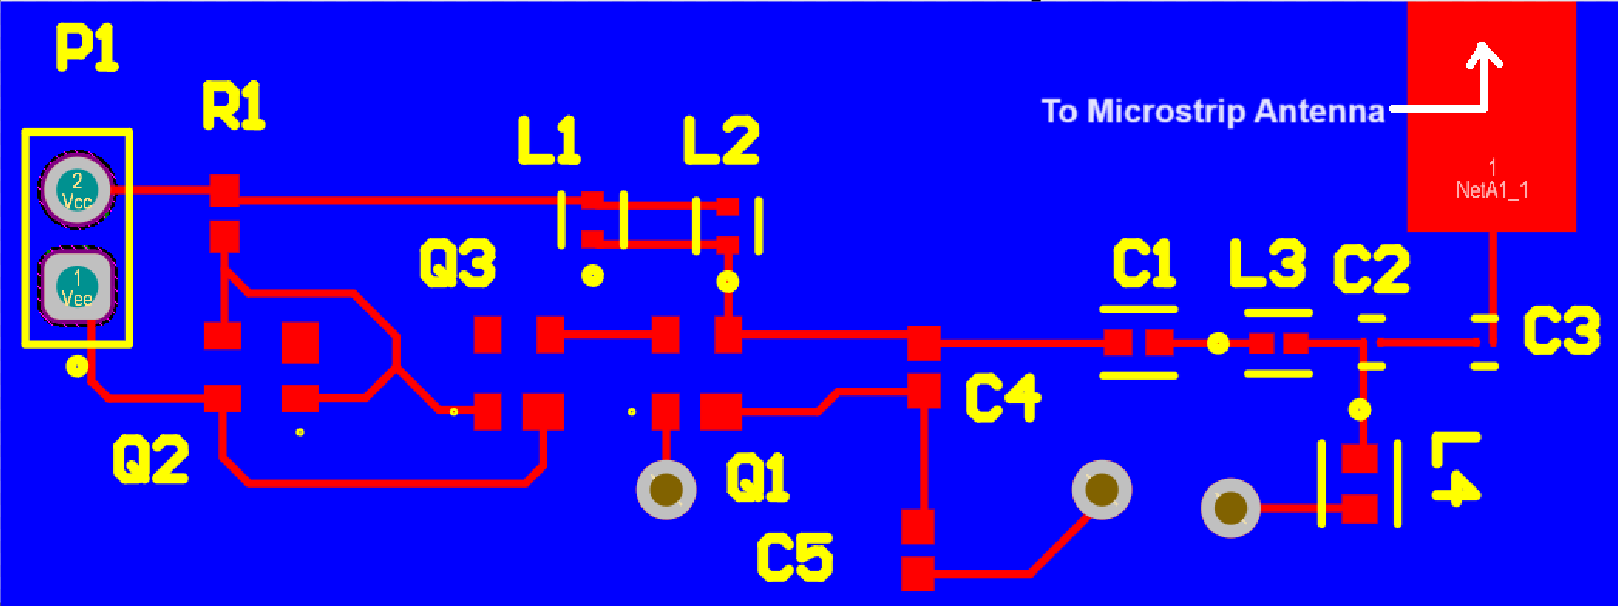
\includegraphics[width=0.9\textwidth]{images/layout/board.png}
    \caption{Altium Board Layout}
    \label{fig:board}
\end{figure}
The circuit was sent to JLC-PCB for fabrication and will be spectrally tested in the RFIC lab. The spectrum of the transmitted output should be a single spike in the frequency domain at \(3.5[GHz]\).